% =========================================================
% Anhang (article-kompatibel)
% =========================================================
% Hinweis: Die gewünschte Struktur verwendet \chapter. Da diese
% Arbeit die article-Klasse nutzt, sind die Kapitel als \section
% (durch \appendix als A, B, C ... nummeriert) und die inneren
% Abschnitte als \subsection umgesetzt.
%
% Werte stammen, soweit vorhanden, aus der tatsächlichen Konfiguration
% des Projekts (args.yaml, Pipeline-Skripte, Tracking-Reports).
% Wo konkrete Werte fehlen, sind Platzhalter wie [ANZAHL] eingetragen.

\clearpage
\appendix
\renewcommand{\appendixname}{Anhang}
\renewcommand{\appendixpagename}{Anhang}
\renewcommand{\appendixtocname}{Anhang}
\addappheadtotoc
\appendixpage

% Unterabschnitte des Anhangs wieder im Inhaltsverzeichnis anzeigen
\addtocontents{toc}{\protect\setcounter{tocdepth}{2}}

% Platzhalter-Box für noch nicht vorhandene Abbildungen (kompiliert ohne Bilddatei)
\newcommand{\anhangplaceholder}[1]{%
    \fbox{\parbox[c][5cm][c]{0.9\textwidth}{%
        \centering\itshape Platzhalter für Abbildung --- Pfad einfügen: \texttt{#1}}}}


% =========================================================
\section{Zusätzliche Materialien zum Datensatzkapitel}
\label{app:datensatz}

Dieser Anhang enthält ergänzende Informationen zum verwendeten Datensatz.
Die hier zusammengestellten Details vertiefen das Datensatzkapitel
(Abschnitt~\ref{sec:datasets}) des Haupttextes, ohne dieses mit umfangreichen
Tabellen und Einzelwerten zu überladen. Sie dienen der Nachvollziehbarkeit und
Reproduzierbarkeit der durchgeführten Experimente.

\subsection{Übersicht der verwendeten Videodaten}

Die folgende Tabelle gibt einen Überblick über die im Rahmen dieser Arbeit
verwendeten Videosequenzen sowie über den Umfang der daraus extrahierten,
manuell annotierten und automatisch erzeugten Daten. Etwa jeder 30.~Frame eines
Videos wurde manuell annotiert; die übrigen Frames wurden zunächst nicht
annotiert.

\begin{table}[htbp]
    \centering
    \caption{Übersicht der verwendeten Videodaten sowie der zugehörigen
    manuellen und automatisch erzeugten Annotationen.}
    \label{tab:anhang_videouebersicht}
    \resizebox{\textwidth}{!}{%
    \begin{tabular}{lccccl}
        \toprule
        \textbf{Video} & \textbf{Extrahierte Frames} &
        \textbf{Manuell annot. Frames} & \textbf{Manuelle Annotationen} &
        \textbf{Pseudo-Labels} & \textbf{Bemerkung} \\
        \midrule
        video01\_regionA & [ANZAHL] & [ANZAHL] & [ANZAHL] & [ANZAHL] & [BEMERKUNG] \\
        video02\_regionA & [ANZAHL] & [ANZAHL] & [ANZAHL] & [ANZAHL] & [BEMERKUNG] \\
        video03\_regionB & [ANZAHL] & [ANZAHL] & [ANZAHL] & [ANZAHL] & [BEMERKUNG] \\
        video04\_regionB & 6285     & [ANZAHL] & [ANZAHL] & [ANZAHL] & Tracking-Beispiel \\
        \multicolumn{6}{c}{\dots} \\
        \midrule
        \textbf{Gesamt (26 Videos)} & [ANZAHL] & [ANZAHL] & [ANZAHL] & [ANZAHL] & \\
        \bottomrule
    \end{tabular}%
    }
\end{table}

\subsection{Aufteilung des Datensatzes}

Der Datensatz wurde in einen Trainings- und einen Validierungsteil aufgeteilt.
Die Aufteilung erfolgte reproduzierbar mit festem Zufallsseed im Verhältnis von
80~\% zu 20~\%. Der Trainingsteil dient der Modellanpassung, der
Validierungsteil der Überwachung des Trainingsverlaufs und der abschließenden,
ausschließlich auf manuellen Annotationen basierenden Bewertung. Ein separater
Testteil wurde in dieser Arbeit nicht gebildet.

\begin{table}[htbp]
    \centering
    \caption{Aufteilung des Datensatzes in Trainings- und Validierungsdaten
    (Verhältnis 80/20).}
    \label{tab:anhang_split}
    \begin{tabular}{lccc}
        \toprule
        \textbf{Split} & \textbf{Frames} & \textbf{Annotationen} & \textbf{Anteil} \\
        \midrule
        Training     & [ANZAHL] & [ANZAHL] & 80\,\% \\
        Validierung  & [ANZAHL] & [ANZAHL] & 20\,\% \\
        Test         & --       & --       & nicht verwendet \\
        \midrule
        \textbf{Gesamt} & [ANZAHL] & [ANZAHL] & 100\,\% \\
        \bottomrule
    \end{tabular}
\end{table}

\subsection{Verteilung der Annotationen}

Manuelle Annotationen und automatisch erzeugte Pseudo-Labels werden getrennt
betrachtet, um den Beitrag der halbüberwachten Annotation transparent zu machen.
Die Pseudo-Labels werden sowohl vor als auch nach der Filterung ausgewiesen. Für
die Filterung wurde eine minimale Detektionskonfidenz von 0{,}60 verwendet; die
klassenbalancierte Auswahl strebte etwa 800~Instanzen je Klasse an
(maximal 1000~Pseudo-Boxen je Klasse).

\begin{table}[htbp]
    \centering
    \caption{Verteilung der manuellen Annotationen und der automatisch erzeugten
    Pseudo-Labels vor und nach der Filterung.}
    \label{tab:anhang_annotationsverteilung}
    \begin{tabular}{lccl}
        \toprule
        \textbf{Datentyp} & \textbf{Anzahl Frames} &
        \textbf{Anzahl Annotationen} & \textbf{Verwendung} \\
        \midrule
        Manuelle Annotationen              & [ANZAHL] & [ANZAHL] & Training + Validierung \\
        Pseudo-Labels vor Filterung        & [ANZAHL] & [ANZAHL] & Zwischenstand, nicht direkt genutzt \\
        Pseudo-Labels nach Filterung       & [ANZAHL] & [ANZAHL] & Kandidaten für das Training \\
        Für das Training verwendete Labels & [ANZAHL] & [ANZAHL] & manuell + gefilterte Pseudo-Labels \\
        \bottomrule
    \end{tabular}
\end{table}

\subsection{Beispielhafte Annotationen}

Zur qualitativen Veranschaulichung zeigt die folgende Abbildung beispielhafte
Frames mit den zugehörigen Annotationen. Dargestellt werden manuelle
Annotationen, automatisch erzeugte Pseudo-Labels sowie durch Objektverfolgung
unterstützte Label-Propagation.

\begin{figure}[htbp]
    \centering
    \anhangplaceholder{figures/appendix\_dataset\_examples.png}
    \caption{Beispielhafte Frames zur qualitativen Veranschaulichung der
    Annotationen. Gezeigt werden manuelle Annotationen, automatisch erzeugte
    Pseudo-Labels und durch Tracking unterstützte Label-Propagation.}
    \label{fig:anhang_dataset_examples}
\end{figure}


% =========================================================
\section{Zusätzliche Materialien zur Methodik}
\label{app:methodik}

Dieser Anhang dokumentiert die konkreten Konfigurationen und Parameter der
verwendeten Methoden (vgl.\ Abschnitt~\ref{sec:method}). Ziel ist es, die
einzelnen Verarbeitungsschritte reproduzierbar zu machen, ohne den methodischen
Haupttext mit Detailwerten zu überladen.

\subsection{Konfiguration des YOLOv8-Trainings}

Die folgende Tabelle fasst die wichtigsten Parameter der Trainingskonfiguration
des Objekterkennungsmodells zusammen.

\begin{table}[htbp]
    \centering
    \caption{Konfiguration des YOLOv8-Trainings (Baseline).}
    \label{tab:anhang_yolo_config}
    \begin{tabular}{ll}
        \toprule
        \textbf{Parameter} & \textbf{Wert} \\
        \midrule
        Modellvariante        & YOLOv8n (\texttt{yolov8n.pt}) \\
        Bildgröße             & $1024 \times 1024$ \\
        Epochen               & 150 \\
        Batch Size            & 16 \\
        Optimizer             & AdamW \\
        Learning Rate (lr0)   & 0{,}001 \\
        Confidence Threshold  & 0{,}25 (Inferenz) \\
        IoU Threshold (NMS)   & 0{,}7 \\
        \bottomrule
    \end{tabular}
\end{table}

\subsection{Parameter der Pseudo-Label-Generierung}

Bei der automatischen Erzeugung der Pseudo-Labels wurden ausschließlich
Detektionen übernommen, die definierte Schwellenwerte hinsichtlich Konfidenz und
Bounding-Box-Eigenschaften erfüllten. Detektionen unterhalb dieser Schwellen
wurden verworfen, um die Qualität der erzeugten Labels sicherzustellen.

\begin{table}[htbp]
    \centering
    \caption{Parameter der Pseudo-Label-Generierung.}
    \label{tab:anhang_pseudo_params}
    \begin{tabular}{ll}
        \toprule
        \textbf{Parameter} & \textbf{Wert} \\
        \midrule
        Confidence Threshold  & 0{,}25 (Generierung), $\geq$ 0{,}60 (nach Filterung) \\
        IoU Threshold (NMS)   & 0{,}7 \\
        Minimale Boxgröße     & normierte Fläche $\geq 1\cdot10^{-6}$ \\
        Maximale Boxgröße     & keine explizite Obergrenze \\
        Verwendetes Modell    & Baseline-YOLOv8n (\texttt{best.pt}) \\
        Bemerkung             & nur Zielklassen; klassenbalancierte Auswahl (Quota) \\
        \bottomrule
    \end{tabular}
\end{table}

\subsection{Parameter des Trackings}

Zur zeitlichen Zuordnung von Detektionen in aufeinanderfolgenden Frames wurde
das Tracking-Verfahren ByteTrack eingesetzt. Dadurch können Objekte über mehrere
Frames hinweg konsistent verfolgt und die resultierenden Trajektorien für die
Label-Propagation genutzt werden.

\begin{table}[htbp]
    \centering
    \caption{Parameter des verwendeten Tracking-Verfahrens (ByteTrack).}
    \label{tab:anhang_tracking_params}
    \begin{tabular}{ll}
        \toprule
        \textbf{Parameter} & \textbf{Wert} \\
        \midrule
        Tracker          & ByteTrack (\texttt{bytetrack.yaml}) \\
        Track Threshold  & 0{,}25 (Eingangs-Detektionsschwelle) \\
        Match Threshold  & [WERT] (Standardwert \texttt{bytetrack.yaml}) \\
        Track Buffer     & [WERT] (Standardwert \texttt{bytetrack.yaml}) \\
        Frame Rate       & 29{,}97 FPS (Beispielvideo \texttt{video04\_regionB}) \\
        Bemerkung        & Standardkonfiguration; \texttt{persist=True} \\
        \bottomrule
    \end{tabular}
\end{table}

\subsection{Verzeichnisstruktur}

Die folgende, beispielhafte Verzeichnisstruktur veranschaulicht die Organisation
der Daten und Zwischenergebnisse innerhalb des Projekts.

\begin{verbatim}
data/
    frames/
    labels/
    pseudo_labels/
    tracking/
runs/
scripts/
README.md
\end{verbatim}


% =========================================================
\section{Zusätzliche Ergebnisse}
\label{app:ergebnisse}

Dieser Anhang enthält ergänzende Ergebnisdarstellungen, die die im
Ergebniskapitel (Abschnitt~\ref{sec:experiments}) getroffenen Aussagen visuell
untermauern. Die Abbildungen dienen der vertiefenden Betrachtung und ergänzen
die im Haupttext gezeigten Auswertungen.

\subsection{Ergänzende Trainingskurven}

Die folgende Abbildung zeigt ergänzende Verläufe der Trainings- und
Validierungsmetriken über die Epochen. Sie veranschaulicht das
Konvergenzverhalten des Modells während des Trainings.

% Alternativ vorhanden: figures/baseline/BoxP_curve.png, figures/baseline/BoxR_curve.png
\begin{figure}[htbp]
    \centering
    \anhangplaceholder{figures/appendix\_training\_curves.png}
    \caption{Ergänzende Trainings- und Validierungskurven über den
    Trainingsverlauf.}
    \label{fig:anhang_training_curves}
\end{figure}

\subsection{Ergänzende Konfusionsmatrizen}

Die folgende Abbildung zeigt ergänzende Konfusionsmatrizen, die das
Klassifikationsverhalten des Modells über die betrachteten Klassen hinweg
darstellen und typische Verwechslungen zwischen Klassen sichtbar machen.

\begin{figure}[htbp]
    \centering
    \anhangplaceholder{figures/appendix\_confusion\_matrix.png}
    \caption{Ergänzende Konfusionsmatrix zur Analyse des
    Klassifikationsverhaltens des Modells.}
    \label{fig:anhang_confusion_matrix}
\end{figure}

\subsection{Beispiele erfolgreicher und fehlerhafter Detektionen}

Die folgende Abbildung zeigt beispielhafte Detektionsergebnisse auf
Validierungsdaten. Neben korrekt erkannten Objekten werden auch typische
Fehlerfälle sichtbar, wodurch Stärken und Grenzen des Modells qualitativ
veranschaulicht werden.

\begin{figure}[htbp]
    \centering
    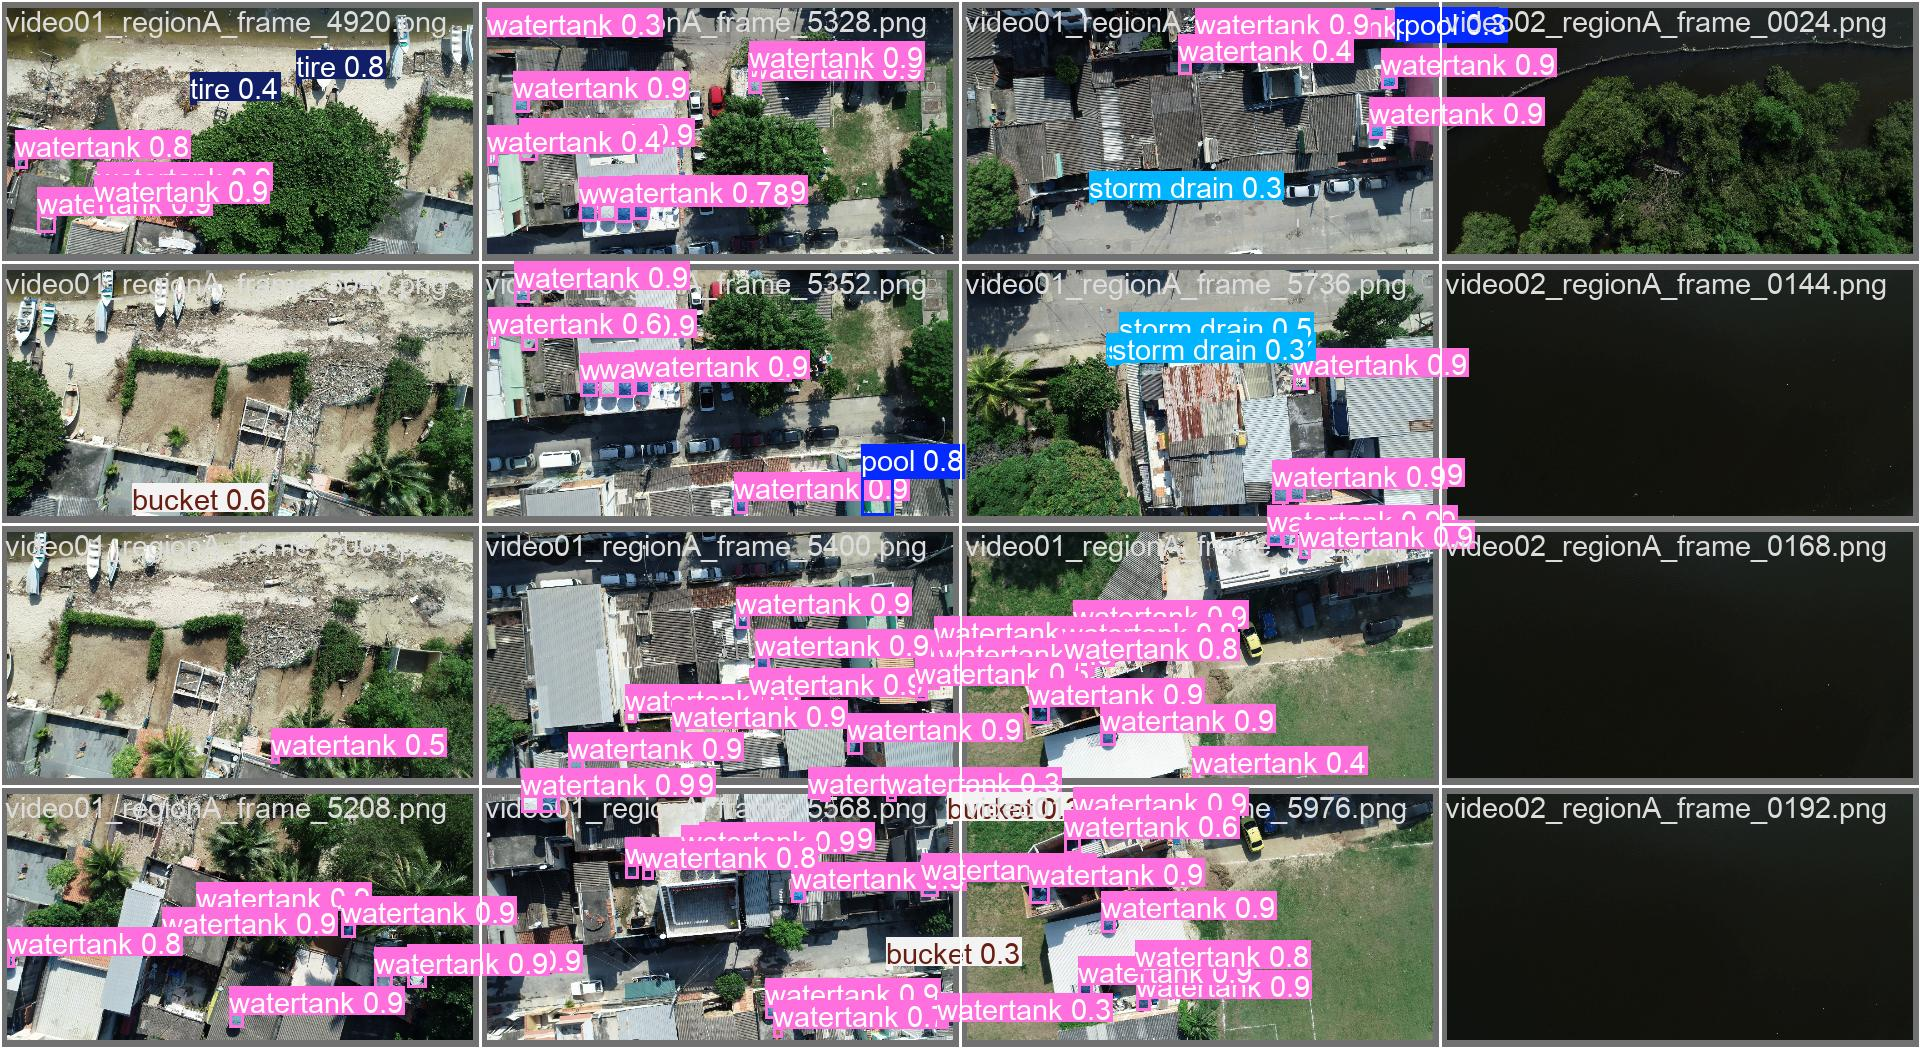
\includegraphics[width=\textwidth]{figures/baseline/val_batch1_pred.jpg}
    \caption{Beispiele erfolgreicher und fehlerhafter Detektionen des
    Baseline-Modells auf einem Validierungsstapel.}
    \label{fig:anhang_detection_examples}
\end{figure}

\subsection{Beispiele der Tracking-basierten Label-Propagation}

Die folgende Abbildung veranschaulicht die tracking-basierte Label-Propagation
über aufeinanderfolgende Frames. Dargestellt wird, wie Detektionen mithilfe der
Objektverfolgung zeitlich verknüpft und als Grundlage für die Erzeugung
zusätzlicher Labels genutzt werden.

% Alternativ vorhanden: figures/tracking/tracking_frame1.jpeg, figures/tracking/tracking_frame2.jpeg
\begin{figure}[htbp]
    \centering
    \anhangplaceholder{figures/appendix\_tracking\_propagation.png}
    \caption{Beispiele der tracking-basierten Label-Propagation über
    aufeinanderfolgende Frames.}
    \label{fig:anhang_tracking_propagation}
\end{figure}


% =========================================================
\section{Quellcode und Reproduzierbarkeit}
\label{app:quellcode}

Der im Rahmen dieser Arbeit entwickelte Quellcode wurde zusammen mit der
digitalen Abgabe bereitgestellt und ist zusätzlich öffentlich unter
\url{https://github.com/Berkekrd/semi-supervised-drone-annotation} verfügbar.
Er umfasst Skripte zur Datenvorverarbeitung, zur Generierung der Pseudo-Labels,
zum Objekttracking, zum Training des Modells sowie zur Evaluation der Ergebnisse.

Die wichtigsten Ausführungsschritte sowie die benötigten Abhängigkeiten sind in
der beiliegenden README-Datei dokumentiert. Die abgegebene Version des
Quellcodes entspricht dem Stand, der für die in dieser Arbeit beschriebenen
Experimente verwendet wurde. Auf die vollständige Wiedergabe des Quellcodes
innerhalb der Arbeit wird bewusst verzichtet; stattdessen wird auf die digitale
Abgabe verwiesen.

Die folgende, beispielhafte Verzeichnisstruktur gibt einen Überblick über die
Organisation des bereitgestellten Quellcodes.

\begin{verbatim}
semi-supervised-drone-annotation/
    scripts/            # Pipeline als Skripte (main1.py ... main18.py)
    notebooks/          # pipeline.ipynb (gesamte Pipeline)
    results/            # Tracking-Ergebnisse (CSV, Reports)
    thesis/             # LaTeX-Quellen der Arbeit
    Readme.md
\end{verbatim}


% =========================================================
\section*{Eigenständigkeitserklärung}
\addcontentsline{toc}{section}{Eigenständigkeitserklärung}

Hiermit erkläre ich, dass ich die vorliegende Arbeit selbstständig und ohne
unzulässige fremde Hilfe verfasst habe. Es wurden keine anderen als die
angegebenen Quellen und Hilfsmittel benutzt. Alle Stellen der Arbeit, die
wörtlich oder sinngemäß aus anderen Quellen übernommen wurden, sind als solche
kenntlich gemacht. Die Arbeit wurde in gleicher oder ähnlicher Form noch keiner
anderen Prüfungsbehörde vorgelegt und auch nicht veröffentlicht.

\vspace{2cm}

\noindent
\begin{tabular}{@{}p{6cm}@{\hspace{2cm}}p{6cm}@{}}
    \hrulefill & \hrulefill \\
    {[ORT], [DATUM]} & {[VORNAME NACHNAME]} \\
\end{tabular}

\newpage
\MSonehalfspacing
